\part{Vectors}
\frame{\partpage}

\newcommand{\cvec}[2]{\begin{pmatrix}#1\\#2\end{pmatrix}}

\begin{frame}{2D vectors}
    \begin{itemize}
        \pause\item A \textbf{2D vector} is represented by a \textbf{pair} of \textbf{numbers}
        \pause\item Often represented as a \textbf{column vector}
        \pause\item E.g.\ $\cvec{3}{2}$ or $\cvec{0}{-4}$ or $\cvec{-3.7}{6.2}$
        \pause\item General form: $\cvec{x}{y}$
        \pause\item Can also have $3, 4, 5, \dots$ dimensional vectors
    \end{itemize}
\end{frame}

\begin{frame}{Vectors as points}
    \begin{itemize}
        \pause\item $\cvec{0}{0}$ is the \textbf{origin}
        \pause\item $\cvec{x}{y}$ represents a point $x$ units to the right and $y$ units up from the origin
            \begin{itemize}
                \pause\item Negative values represent left and down
                \pause\item In computer graphics, sometimes $y$ points down instead of up
            \end{itemize}
    \end{itemize}
\end{frame}

\begin{frame}{Operations on vectors}
    \begin{itemize}
        \pause\item Addition and subtraction work \textbf{element-wise}
            \begin{itemize}
                \pause\item $\cvec{x_1}{y_1} + \cvec{x_2}{y_2} = \cvec{x_1+x_2}{y_1+y_2}$
                \pause\item $\cvec{x_1}{y_1} - \cvec{x_2}{y_2} = \cvec{x_1-x_2}{y_1-y_2}$
            \end{itemize}
        \pause\item Multiplication by a \textbf{scalar} (a number) also works element-wise
            \begin{itemize}
                \pause\item $c \times \cvec{x}{y} = \cvec{c \times x}{c \times y}$
            \end{itemize}
    \end{itemize}
\end{frame}

\begin{frame}{Vectors as offsets}
    \begin{itemize}
        \pause\item $\cvec{x}{y}$ represents an offset of $x$ units to the right and $y$ units up
        \pause\item Subtraction: if $p$ and $q$ are points, then $q-p$ is the offset of $q$ relative to $p$
        \pause\item Addition: if $p$ is a point and $u$ is an offset, then $p+u$ is the point at an offset of $u$ from $p$
        \pause\item Addition: if $u$ and $v$ are offsets, then $u+v$ is the combined offset
    \end{itemize}
\end{frame}

\begin{frame}{Trigonometry}
	\begin{columns}
		\begin{column}{0.48\textwidth}
			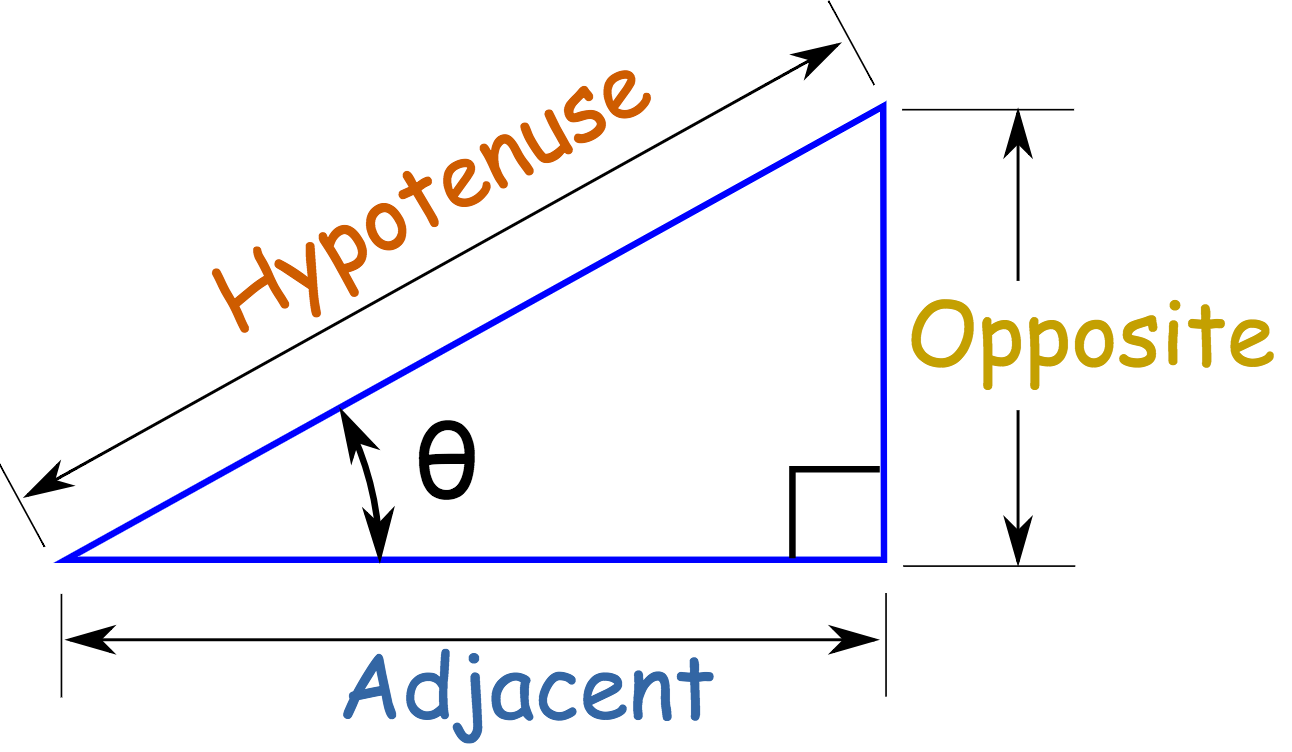
\includegraphics[width=\textwidth]{right_triangle}
		\end{column}
		\begin{column}{0.48\textwidth}
		    \begin{itemize}
		        \pause\item $\operatorname{sin} \theta = \frac{\operatorname{opposite}}{\operatorname{hypotenuse}}$
		        \pause\item $\operatorname{cos} \theta = \frac{\operatorname{adjacent}}{\operatorname{hypotenuse}}$
		        \pause\item $\operatorname{tan} \theta = \frac{\operatorname{opposite}}{\operatorname{adjacent}}$
		    \end{itemize}
		\end{column}
	\end{columns}
\end{frame}

\begin{frame}{Sine, cosine and tangent}
    \begin{center}
    	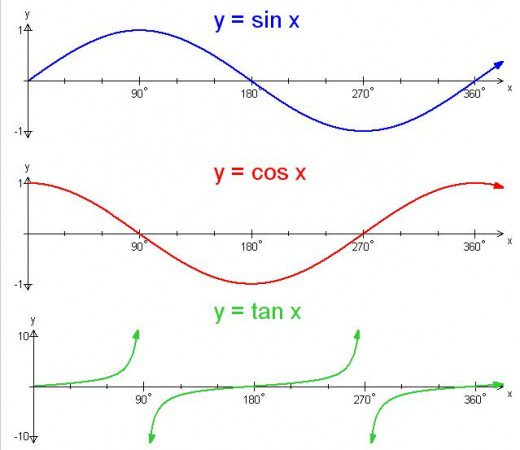
\includegraphics[width=0.8\textheight]{sin_cos_tan_graph}
	\end{center}
\end{frame}

\begin{frame}{Radians}
	\begin{itemize}
		\pause\item We often measure angles in \textbf{radians}
		\pause\item $\pi = 3.14159\dots$ 
		\pause\item $\pi \text{ radians} = 180 \text{ degrees} = \text{half a circle}$ 
		\pause\item $\frac{\pi}{2} \text{ radians} = 90 \text{ degrees} = \text{right angle}$
	\end{itemize}
\end{frame}

\begin{frame}{Magnitude and direction}
	\begin{columns}
		\begin{column}{0.48\textwidth}
			\pause A vector has \textbf{components}
			\pause 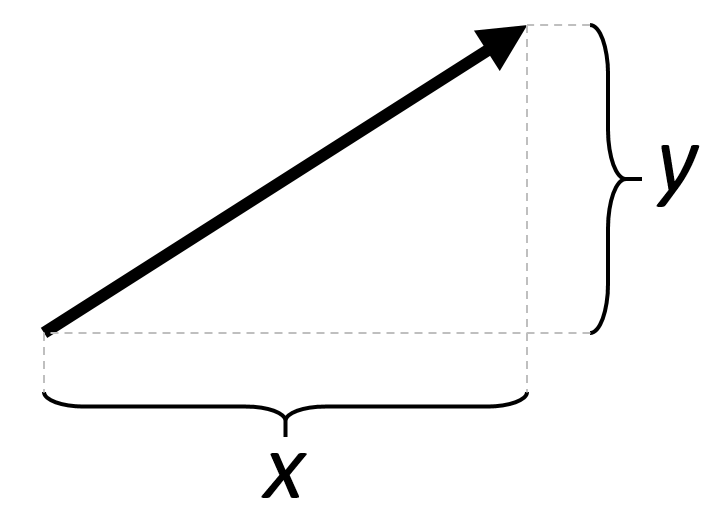
\includegraphics[width=\textwidth]{vector_components}
		\end{column}
		\begin{column}{0.48\textwidth}
			\pause A vector also has \textbf{direction} and \textbf{magnitude} (or \textbf{length})
			\pause 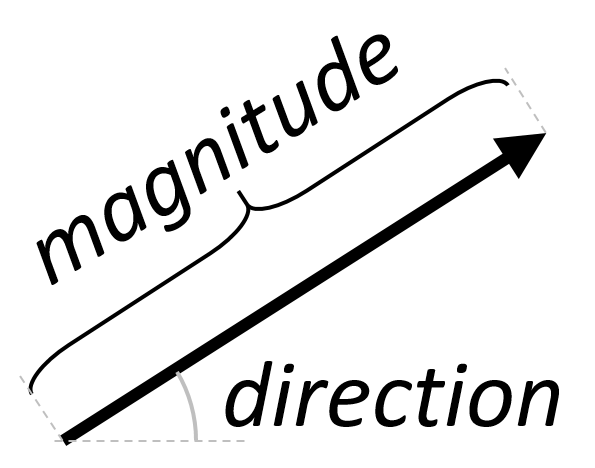
\includegraphics[width=\textwidth]{vector_polar}
			
			\pause (Direction is measured as an angle from the positive $x$-axis)
		\end{column}
	\end{columns}
\end{frame}

\begin{frame}{Magnitude and direction}
    \begin{itemize}
        \pause\item The magnitude of $\cvec{x}{y}$ is $\sqrt{x^2 + y^2}$
        \pause\item The direction of $\cvec{x}{y}$ is $\operatorname{tan}^{-1} \left( \frac{y}{x} \right)$
        \pause\item The vector with magnitude $r$ and direction $\theta$ is
            $\cvec{r \operatorname{cos} \theta}{r \operatorname{sin} \theta}$
        \pause\item Multiplication: if $u$ is a vector with magnitude $r$ and direction $\theta$,
            then $c \times u$ has magnitude $c \times r$ and direction $\theta$
    \end{itemize}
\end{frame}

